\documentclass[11pt]{article}
\usepackage{graphics}
\usepackage{amsthm}
\usepackage{amsmath}
\usepackage{amssymb}
\usepackage{bm}
\usepackage{amsbsy}
\usepackage{mathtools}
\usepackage{algpseudocode, algorithm, algorithmicx}
\usepackage{soul}
\usepackage{graphicx}
\usepackage{color}
\usepackage{float}
\usepackage{gensymb}
\usepackage{tabularx}
\newcommand{\ord}[1]{\textsuperscript{#1}}
\usepackage{ragged2e}
\DeclareMathOperator{\DICT}{DICT}


\graphicspath{ {./images/HW5/} }

\makeatletter
\DeclareFontFamily{U}{tipa}{}
\DeclareFontShape{U}{tipa}{m}{n}{<->tipa10}{}
\newcommand{\arc@char}{{\usefont{U}{tipa}{m}{n}\symbol{62}}}%

\newcommand{\arc}[1]{\mathpalette\arc@arc{#1}}

\newcommand{\arc@arc}[2]{%
  \sbox0{$\m@th#1#2$}%
  \vbox{
    \hbox{\resizebox{\wd0}{\height}{\arc@char}}
    \nointerlineskip
    \box0
  }%
}
\makeatother

\makeatletter
\newcommand\multiline[1]{\parbox[t]{\dimexpr\linewidth-\ALG@thistlm}{#1}}
\makeatother
\usepackage[margin=1in]{geometry}
%\renewcommand{\baselinestretch}{1.2}
\newcommand{\codepar}[2]{\begin{minipage}[t]{#1}#2\end{minipage}}
\newcommand{\codecomt}[1]{\color{blue}\textit{// #1}\color{black}}

% You can put more user-defined commands here

\makeatletter
\newlength{\continueindent}
\setlength{\continueindent}{6em}

\renewenvironment{algorithmic}[1][0]%
   {%
   \edef\ALG@numberfreq{#1}%
   \def\@currentlabel{\theALG@line}%
   %
   \setcounter{ALG@line}{0}%
   \setcounter{ALG@rem}{0}%
   %
   \let\\\algbreak%
   %
   \expandafter\edef\csname ALG@currentblock@\theALG@nested\endcsname{0}%
   \expandafter\let\csname ALG@currentlifetime@\theALG@nested\endcsname\relax%
   %
   \begin{list}%
      {\ALG@step}%
      {%
      \rightmargin\z@%
      \itemsep\z@ \itemindent\z@ \listparindent2em%
      \partopsep\z@ \parskip\z@ \parsep\z@%
      \labelsep 0.5em \topsep 0.2em%\skip 1.2em 
      \ifthenelse{\equal{#1}{0}}%
         {\labelwidth 0.5em}%
         {\labelwidth 1.2em}%
       \leftmargin\labelwidth \addtolength{\leftmargin}{\labelsep}
      \ALG@tlm\z@%
      }%
      \parshape 2 \leftmargin \linewidth \continueindent \dimexpr\linewidth-\continueindent\relax
   \setcounter{ALG@nested}{0}%
   \ALG@beginalgorithmic%
   }%
   {% end{algorithmic}
   % check if all blocks are closed
   \ALG@closeloops%
   \expandafter\ifnum\csname ALG@currentblock@\theALG@nested\endcsname=0\relax%
   \else%
      \PackageError{algorithmicx}{Some blocks are not closed!!!}{}%
   \fi%
   \ALG@endalgorithmic%
   \end{list}%
   }%
\makeatother

\newcommand{\CH}{\mathrm{CH}}
\renewcommand{\thealgorithm}{}

\newenvironment{solution}
  {\renewcommand\qedsymbol{$\blacksquare$}\begin{proof}[Solution]}
  {\end{proof}}
  
\begin{document}

\hrule
\begin{center}
    \textbf{CS91T: Computational Geometry}\hfill \textbf{Fall 2023}\newline

    {\Large Homework 7}

    David Yang and Nick Fettig
\end{center}

\hrule

\vspace{1em}

\begin{enumerate}
\item{\textbf{Let $P$ be a set of $n$ points in the plane. Give an $O(n\log n)$-time algorithm to find, for each point $p\in P$, another point in $P$ that is closest to it. Prove that your algorithm is correct and achieves the stated running time.}}

\begin{minipage}[t]{0.9\textwidth}
    \begin{algorithm}[H]
    \caption{\textsc{ClosestPoints}($P$)}
    \begin{algorithmic}[1]
        \State{Set $E\coloneqq$ \textsc{Vor}($P$)}\footnotemark
        \State{Set $closest\coloneqq$ dictionary with a key for each $p\in P$ and all values initialized to \textsc{Null}}
        \For{each edge $(v_1, v_2) \in E$}
            \If{$closest[v_1] == \textsc{Null}$ OR $||\overline{v_1v_2}|| < || \overline{(v_1, closest[v_1])}||$ }
                \State{Set $closest[v_1] = v_2$}
            \EndIf
            \If{$closest[v_2] == \textsc{Null}$ OR $||\overline{v_1v_2}|| < ||\overline{(v_2, closest[v_2])}||$ }
                \State{Set $closest[v_2] = v_1$}
            \EndIf
        \EndFor
        \State{\textbf{return} $closest$} 
    \end{algorithmic}
    \end{algorithm}
\end{minipage}


\footnotetext{\textsc{Vor} is a function that generates the Voronoi Diagram for a point set $P$, a modified version of Fortune's Algorithm. It will return the edge set (in adjacency list form) for $\mathcal{V}(P)$, with the extra condition that each edge holds the two vertices in $P$ it separates.}

\vspace{1em}

\textbf{Runtime Analysis}: Line 1 calls \textsc{Vor}, our function to find the Voronoi diagram of a point set $P$. Since \textsc{Vor} is a modification of Fortune's algorithm with the extra condition that each edge returned by \textsc{Vor} contains the two sites it separates (which can be done without any extra work in Fortune's algorithm), it runs in $O(n\log n)$-time. On line 2, we also initialize a dictionary in $O(n)$-time, setting up a key-value pair for each of the $n$ points in $P$. \\

Lines 3-10 run through each edge returned by \textsc{Vor}. The Voronoi diagram can have $O(n)$ edges, so this loop runs $O(n)$ times. Inside the loop, we do a number of constant time comparisons and modifications, checking if any edge yields a closer pair of sites corresponding to neighboring Voronoi cells. We return the $closest$ dictionary at the end, another constant time operation. \\

The total runtime of this algorithm is
\[O(n\log n) + O(n) + O(n)\cdot O(1) = O(n\log n)\]

as desired.

\newpage
\textbf{Proof of Correctness}: Since by definition, the cells of a Voronoi diagram correspond to the region of points closest to each site, the closest point to a point in $P$ must be the site of one of its neighboring cells in the Voronoi diagram. \\

The edges of the Voronoi diagram separate Voronoi cells corresponding to neighboring sites. Consequently, checking for the closest neighbor to each site in $P$ is simple; since we also store information about neighboring vertices in each edge, we find all neighboring sites in the Voronoi diagram by iterating through the entire edge set $E$. We update the closest points to each point in $P$ throughout this process. \\

The correctness of \textsc{Vor} is given to us by the correctness of Fortune's Algorithm. Furthermore, \textsc{ClosestPoints} will correctly keep track of and update the closest points using a dictionary, and thus, the algorithm will correctly find the closest points to each point in $P$.

\newpage
\item\textbf{Let $P$ be any finite set of sites. Prove that for each $p\in P$, the cell $\mathcal{V}(p)$ is unbounded if and only if $p$ is on the boundary of \textsc{CH}($P$).}

\begin{solution}
To prove that for each $p\in P$, the cell $\mathcal{V}(p)$ is unbounded if and only if $p$ is on the boundary of CH($P$), we will prove both directions of the implication. \\

For the forward implication, we will prove the contrapositive: if $p$ is in the convex hull of $P$, then $\mathcal{V}(p)$ is bounded. Let $p$ lie in CH($P$). Consider the ray $r$ starting at $p$ and extending out in any arbitrary direction. Since $p$ is in CH($P$), the ray $r$ must intersect some edge $\overline{xy}$ of the convex hull (with $x, y$ in $P$). Consider the perpendicular bisectors of $\overline{xp}$ and $\overline{yp}$, and let the bases of these perpendicular bisectors be $b_1$ and $b_2$, respectively. By definition, these perpendicular bisectors intersect at a point $c$, the circumcenter of $\triangle pxy.$ By construction, every point outside $\text{CH}(P) \cup \triangle cb_1b_2$ will be closer to $x$ or $y$ than it is to $p$. Since we can construct the ray $r$ in any arbitrary direction, we will find a bounded region in every direction. Consequently, we conclude that the cell $\mathcal{V}(p)$ consisting of points closer to $p$ than any other site, must be bounded. By a proof of the contrapositive, we have resolved the forward implication. \\

For the reverse implication, suppose that $p$ is a point on CH$(P)$. We will split our work into two cases, when $p$ is an intersection of two boundary edges of CH($P$) or when $p$ lies on one such edge. In the former case, consider the perpendicular bisectors of these two edges of CH($P$). By the convexity of CH($P$), these perpendicular bisectors will not intersect outside of CH($P$), and thus, $\mathcal{V}(p)$ will be unbounded. In the latter case, consider the line $\ell$ passing through $p$ that is perpendicular to the boundary edge of CH($P$). Let $r$ be the portion of $\ell$ that lies outside of CH($P$). Due to the Pythagorean Theorem, the closest point in $P$ to each point on $r$ is $p$, and so $r$ must be fully contained in $\mathcal{V}(p)$. Since $r$ extends infinitely, $\mathcal{V}(p)$ is unbounded. \end{solution}

\newpage
\item{\textbf{Suppose you have a Voronoi diagram for some set $P$ of $n$ sites, in the following form:
\begin{itemize}
    \item For each site $p$, a clockwise list of the vertices of $\mathcal{V}$($p$).
    \item For each vertex $v$, a clockwise list of the sites whose cells have $v$ as a vertex.
\end{itemize}
Design an $O(n)$-time algorithm to update the diagram after a new site $q$ is added. Prove that
your algorithm is correct and achieves the stated running time.}} \\

Assume that we are given a set $P$ of $n$ sites, a dictionary $VS$ which stores in $VS[v]$ a clockwise list of sites whose cells have $v$ as a vertex, and a dictionary $SV$ which stores in $SV[p]$ a clockwise list of vertices of $\mathcal{V}(p)$. Additionally, assume we are given the Voronoi diagram of the points in $P$, $\mathcal{V}(P)$, and the new site $q$ to be added.

\begin{minipage}[t]{0.9\textwidth}
    \begin{algorithm}[H]
    \caption{\textsc{UpdatedVoronoi}($P$, $VS$, $SV$, $\mathcal{V}(P)$, $q$)}
    \begin{algorithmic}[1]
        \State{Set $\mathcal{V}(P \cup \{q\}) = \mathcal{V}(P)$}
        \State{Set $p_c \coloneqq$ closest point in $P$ to $q$}
        \State{Set $b \coloneqq$ perpendicular bisector of $\overline{p_cq}$}
        \While{$b$ intersects an edge $e$ in the Voronoi diagram}
            \State{Set $u \coloneqq$ point of intersection of $b$ with $e$}
            \State{Set $c \coloneqq$ the cell that edge $e$ belongs to that does not contain $p_c$}
            \State{Set $p_c \coloneqq$ the site in $P$ corresponding to cell $c$}
            \State{Set $b$ to be the perpendicular bisector of $\overline{p_cq}$}
            \State{Use $u$ to update $VS$, and $SV$ and remove/redefine vertices of $\mathcal{V}(P \cup \{q\})$ as necessary.}
        \EndWhile
        
        \State{\textbf{return} $\mathcal{V}(P \cup \{q\})$} 
    \end{algorithmic}
    \end{algorithm}
\end{minipage}

\vspace{1em}

\textbf{Runtime Analysis}: 
Lines $1$ to $3$ consist of initialization steps. Line $1$ copies the existing Voronoi diagram to our desired output. This will conclude in $O(n)$ time since the Voronoi diagram has $O(n)$ vertices and edges. Line $2$ takes $O(n)$ time to compute; we can simply compare the distances from each of the $n$ sites to $q$ and find the closest site. Finally, line $3$ can be done in constant time. \\

Lines $4$ to $10$ define the main part of the algorithm. Note that the number of iterations of the while loop in line $4$ is at most the number of neighbors of the Voronoi cell containing $q$: $O(n)$ iterations. Each of lines $5$ to $8$ can be done in constant time, using the given information of the Voronoi diagram stored in $VS, SV,$ and $\mathcal{V}(P).$ Finally, the updates in line $9$ can also be done in constant time. Thus, the overall runtime of our algorithm is $O(n)$. \\

\textbf{Proof of Correctness}: We will show that the returned Voronoi diagram is indeed the updated Voronoi diagram, with a new site $q$ added. It is sufficient to show that in each iteration of our while loop, we update a cell to include information about $q$. Consider one such iteration; we will show that the Voronoi cell in the updated Voronoi diagram must contain the point $u$ for the given iteration as its vertex. By construction, each $u$ is the intersection of the perpendicular bisectors between sites of neighboring cells, which is precisely the desired updated Voronoi cell. Thus, our construction works as intended and by iterating through all possible intersections of perpendicular bisectors with existing edges in the Voronoi diagram, we arrive at the desired Voronoi diagram after a new site $q$ is added.

% \begin{itemize}
%     \item Find the closest point in $P$ to $q$ and call this point $p_c$ (linear search: $O(n)$)
%     \item Find all vertices in $\mathcal{V}(p_c)$, that are closer to $q$ than $p_c$ and store them in a list $removed\_v$ as well as remove them from the vertex list  
%     \begin{itemize}
%         \item All vertices we remove will be neighbors of each other by CW nature of list (need to prove)
%         \item Call the vertex to the left of the neighbored vertices we removed $p_l$ and the right vertex $p_r$
%     \end{itemize}
%     \item For each vertex in $removed\_v$... for each site in $removed\_v[i]$:
%     \begin{itemize}
%         \item Find intersection of perpendicular bisectors for each of these vertices as well as the intersection to $p_r + 1$ and $p_l - 1$ (in the list of clockwise vertices of $p_c$)
%         \item save these intersections and their vertices
%         \item also save new vertices and the list of sites 
%     \end{itemize}
% \end{itemize}

\newpage
\item{\textbf{Use a software tool of your choice to make a Voronoi diagram where the sites are the buildings that have vending machines.}}
\vspace{1em}
%https://www.swarthmore.edu/onecard/vending-machines to find vending machines%

\begin{center}
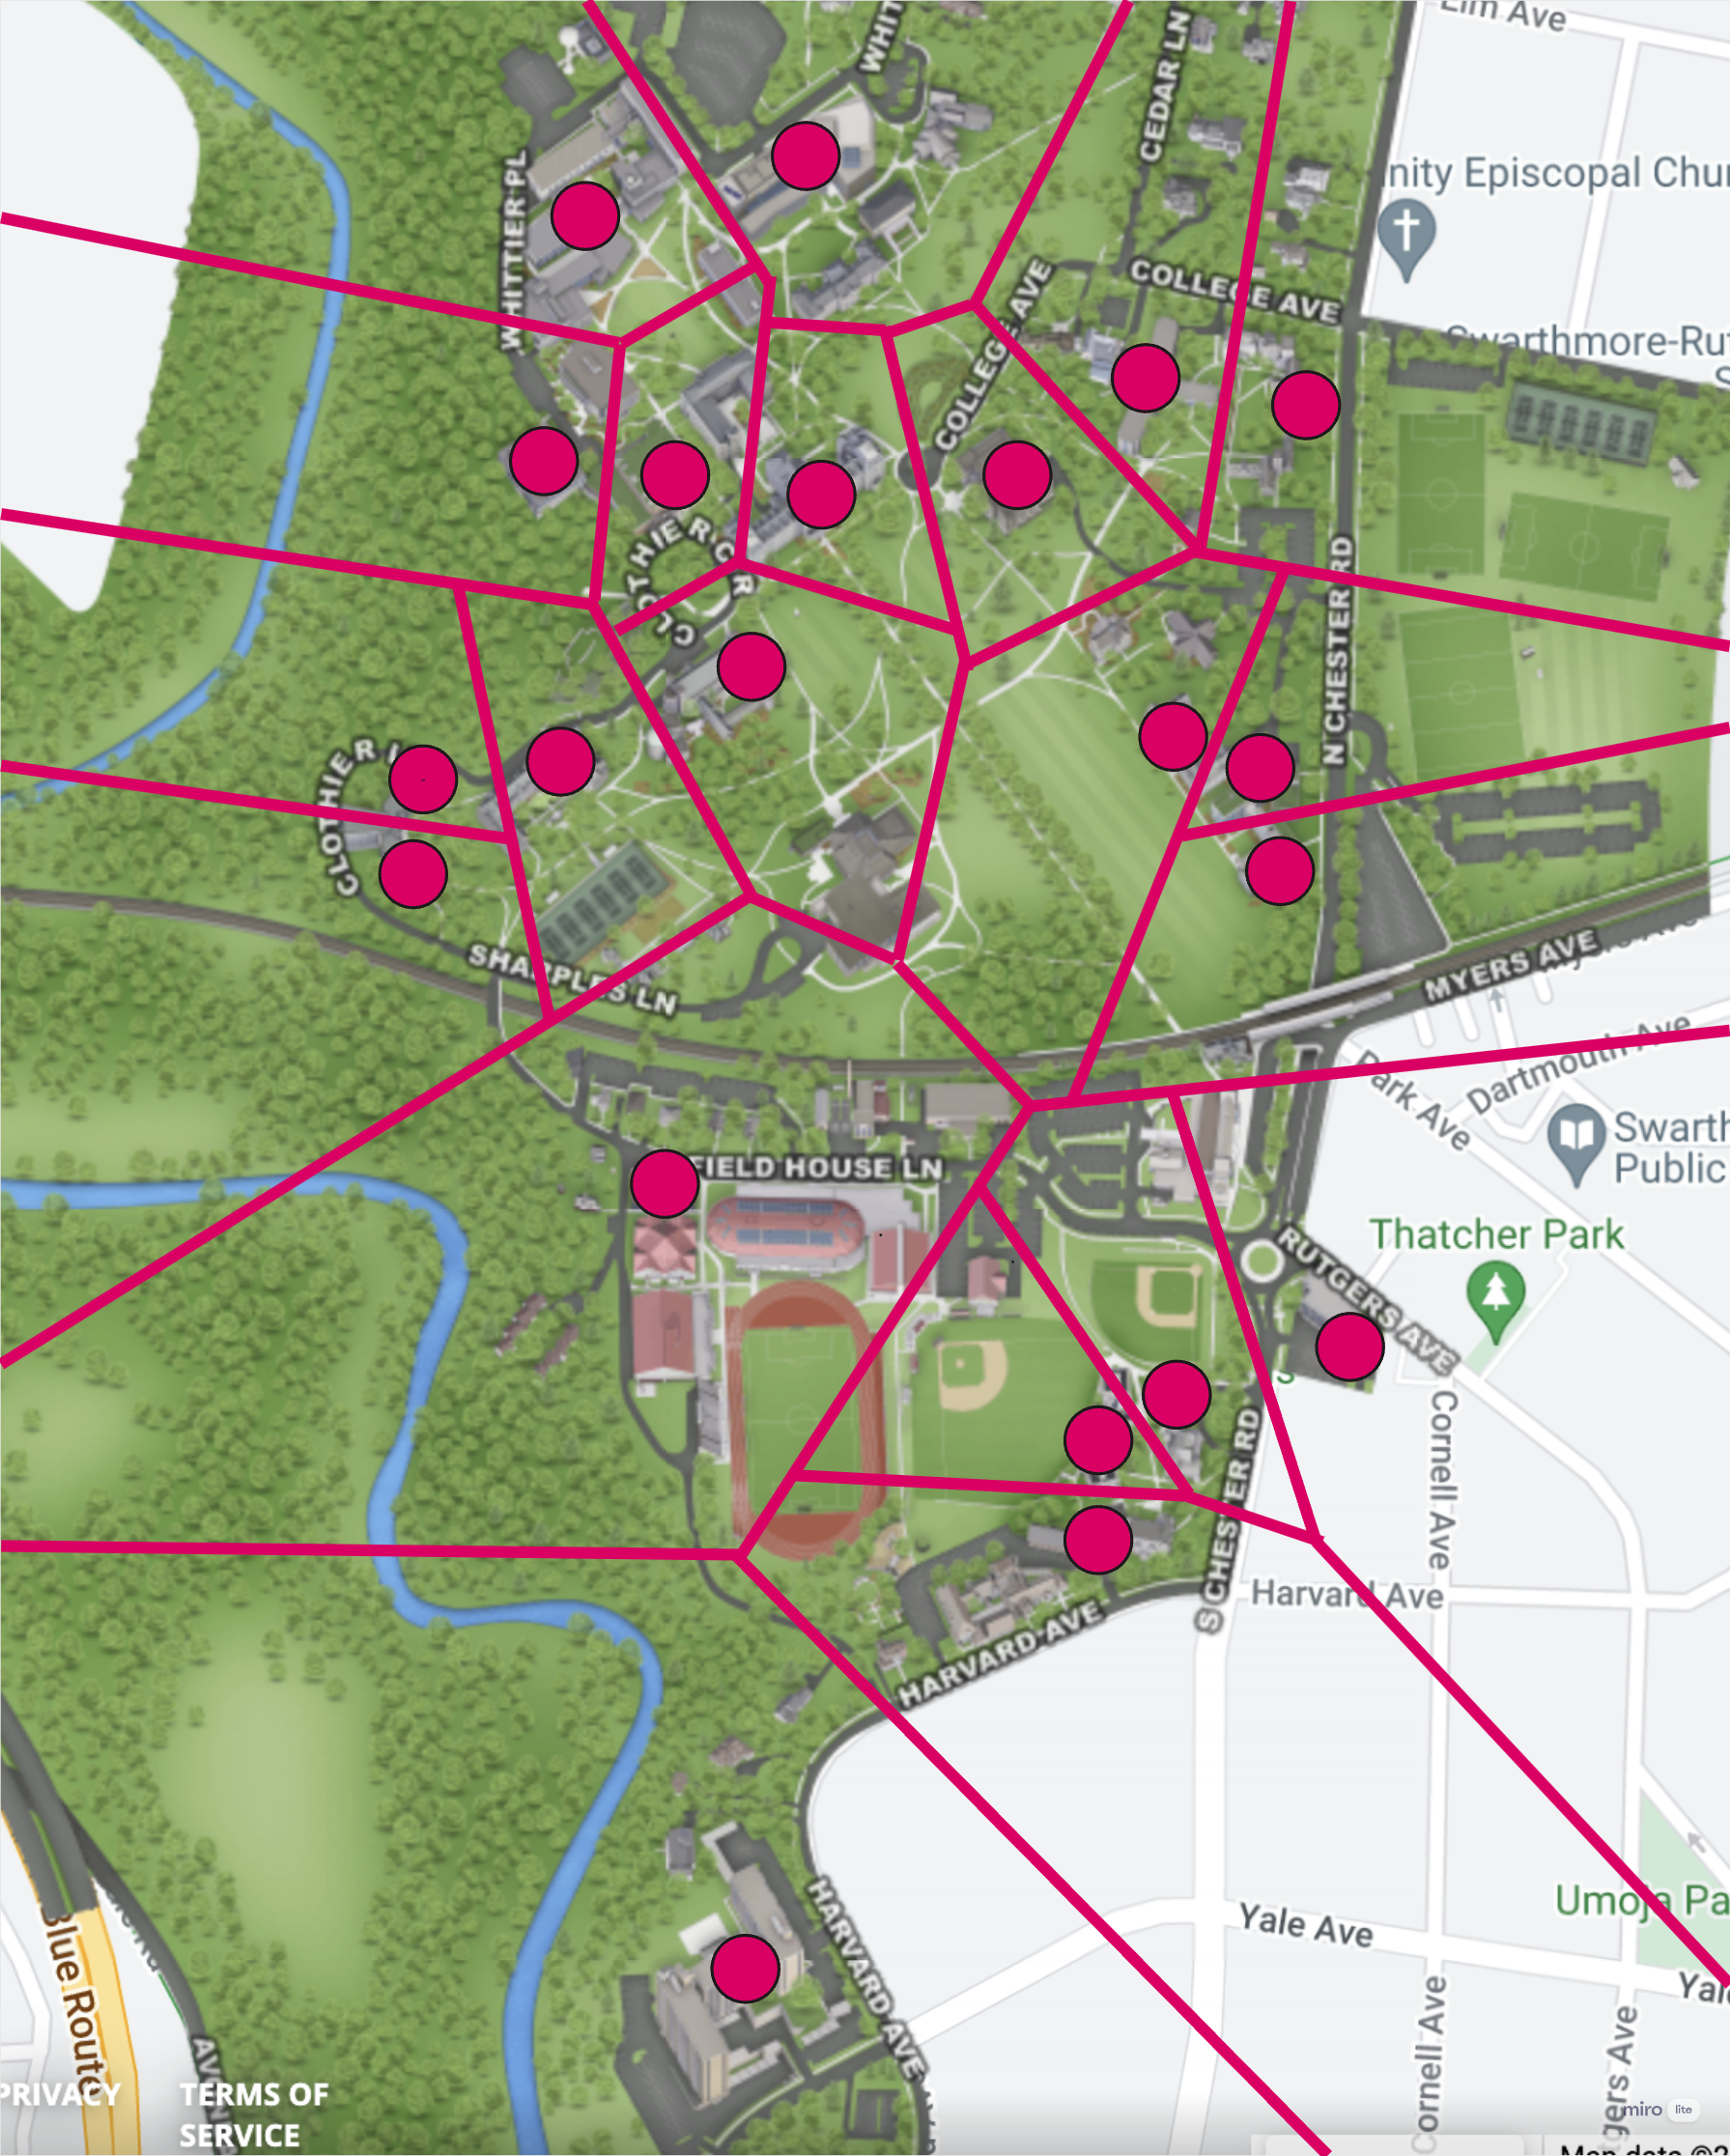
\includegraphics[scale=0.25]{images/HW7/map.png}
\end{center}

\end{enumerate}
\end{document}